%! Author = lili
%! Date = 7/28/26
\chapter{Abgabe 1.2}

\section{HA 1.2.2}
Die Funktion $f:\mathbb R\to\mathbb R$ sei gegeben durch
\[
    f(x)=\begin{cases}
             \dfrac{3|x|}{c} & \text{für } x\in[-1,0], \\[4pt]
             \dfrac{5x^2}{c} & \text{für } x\in[1,5], \\[4pt]
             0 & \text{sonst},
    \end{cases}
\]
wobei $c\in\mathbb R$ eine Konstante sei. Außerdem seien $A_n=\left[1,2-\tfrac1n\right]\subseteq\mathbb R$ für alle $n\in\mathbb N$ und $A=\bigcup_{n\in\mathbb N} A_n$.
\begin{auf}[Bestimmen Sie $c$ so, dass $f$ eine Dichte ist.]
    \textbf{Lösung von mir, Ergebnis überprüft von Tutor.}
    \begin{figure}[H]
        \centering
        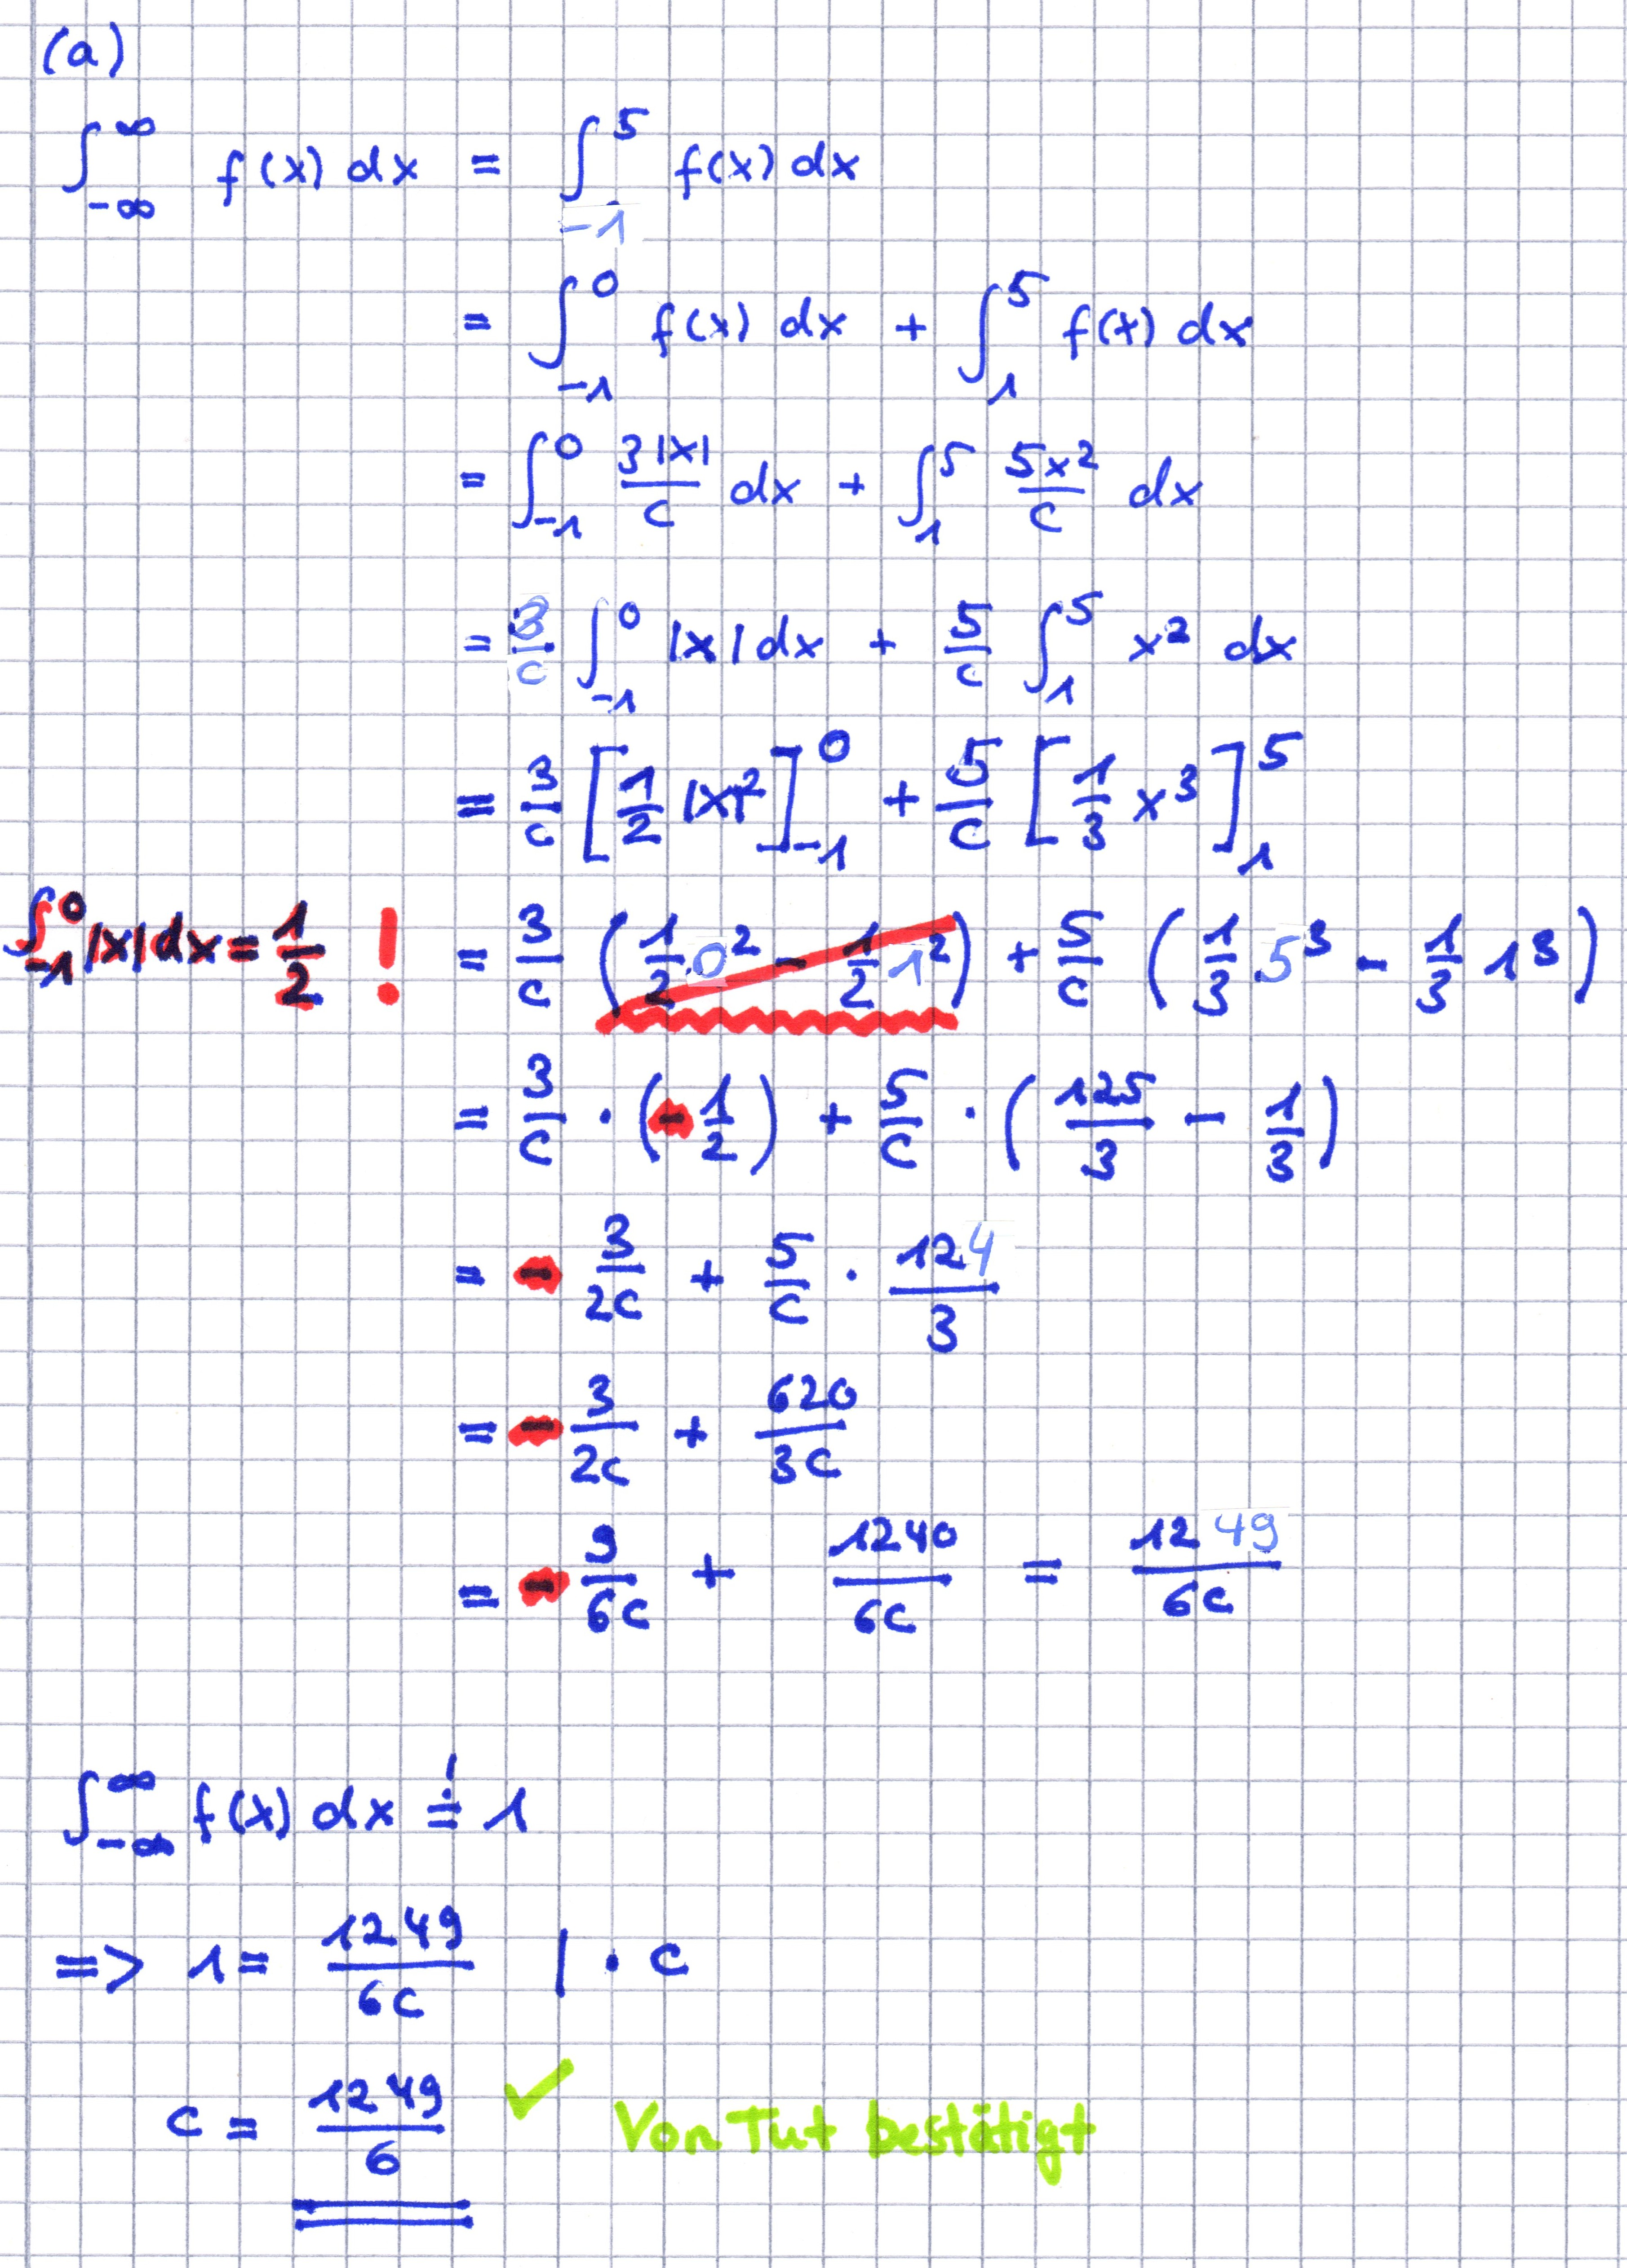
\includegraphics[width=\linewidth]{images/lösungen/wts122a}
    \end{figure}
\end{auf}